\documentclass[border=10pt]{standalone}
\usepackage{tikz}
\usepackage{fontspec}
\usepackage{xcolor}

% Use TeX Gyre Termes (Times clone) which is available in all TeX distributions
\setmainfont{TeX Gyre Termes}
\setsansfont{TeX Gyre Heros}
\setmonofont{TeX Gyre Cursor}

% TikZ libraries
\usetikzlibrary{shapes,arrows,positioning,calc,patterns,decorations.pathreplacing,chains,shadows}
\usetikzlibrary{shapes.geometric,shapes.symbols,shapes.misc}
\usetikzlibrary{matrix,fit,backgrounds}
\usetikzlibrary{arrows.meta}

% Custom colors
\definecolor{bertblue}{RGB}{66,133,244}
\definecolor{gptgreen}{RGB}{52,168,83}
\definecolor{vitpurple}{RGB}{142,36,245}
\definecolor{maskred}{RGB}{234,67,53}
\definecolor{clsorange}{RGB}{251,188,5}
\definecolor{darkgray}{RGB}{50,50,50}
\definecolor{unkred}{RGB}{234,67,53}
\definecolor{subwordpurple}{RGB}{142,36,245}
\definecolor{sepviolet}{RGB}{142,36,245}

\begin{document}
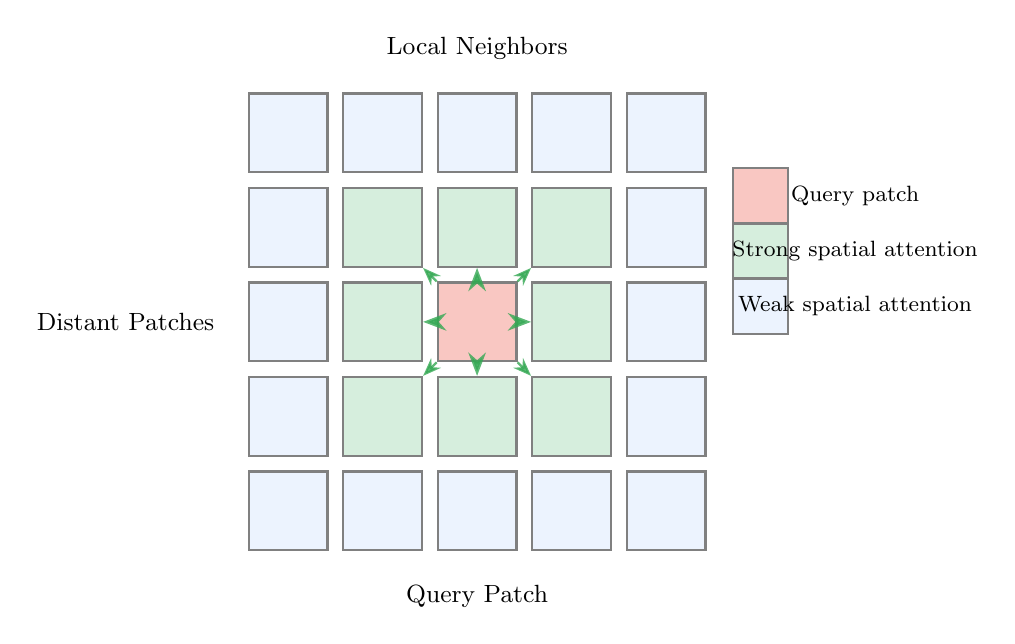
\begin{tikzpicture}[
    patch/.style={rectangle, minimum width=1cm, minimum height=1cm, draw=gray, thick},
    center/.style={patch, fill=maskred!30},
    neighbor/.style={patch, fill=gptgreen!20},
    distant/.style={patch, fill=bertblue!10},
    attention/.style={-{Stealth}, thick, opacity=0.8}
]

% 5x5 grid of patches
\foreach \x in {0,1,2,3,4} {
    \foreach \y in {0,1,2,3,4} {
        \pgfmathsetmacro{\distance}{sqrt((\x-2)*(\x-2) + (\y-2)*(\y-2))}
        \ifnum\x=2
            \ifnum\y=2
                \node[center] (patch\x\y) at (\x*1.2, \y*1.2) {};
            \else
                \ifdim\distance pt<1.5pt
                    \node[neighbor] (patch\x\y) at (\x*1.2, \y*1.2) {};
                \else
                    \node[distant] (patch\x\y) at (\x*1.2, \y*1.2) {};
                \fi
            \fi
        \else
            \ifdim\distance pt<1.5pt
                \node[neighbor] (patch\x\y) at (\x*1.2, \y*1.2) {};
            \else
                \node[distant] (patch\x\y) at (\x*1.2, \y*1.2) {};
            \fi
        \fi
    }
}

% Strong attention to immediate neighbors
\draw[attention, gptgreen, very thick] (patch22) -- (patch12);
\draw[attention, gptgreen, very thick] (patch22) -- (patch32);
\draw[attention, gptgreen, very thick] (patch22) -- (patch21);
\draw[attention, gptgreen, very thick] (patch22) -- (patch23);

% Weaker attention to diagonal neighbors
\draw[attention, gptgreen] (patch22) -- (patch11);
\draw[attention, gptgreen] (patch22) -- (patch13);
\draw[attention, gptgreen] (patch22) -- (patch31);
\draw[attention, gptgreen] (patch22) -- (patch33);

% Labels
\node[font=\small, below=0.3cm of patch20] {Query Patch};
\node[font=\small, above=0.3cm of patch24] {Local Neighbors};
\node[font=\small, left=0.3cm of patch02] {Distant Patches};

% Legend
\node[center, scale=0.7] at (6, 4) {};
\node[font=\footnotesize] at (7.2, 4) {Query patch};
\node[neighbor, scale=0.7] at (6, 3.3) {};
\node[font=\footnotesize] at (7.2, 3.3) {Strong spatial attention};
\node[distant, scale=0.7] at (6, 2.6) {};
\node[font=\footnotesize] at (7.2, 2.6) {Weak spatial attention};

\end{tikzpicture}
\end{document}